\section{General Description}

In this section the general design of the program will be described. In the program there are only one general item, and that is the navigation bar at the bottom. The navigation bar can be seen in all of the figures throughout the design sketch section, as well as in \cref{NavigationBarSketch}

\begin{figure}[H]
	\centering
    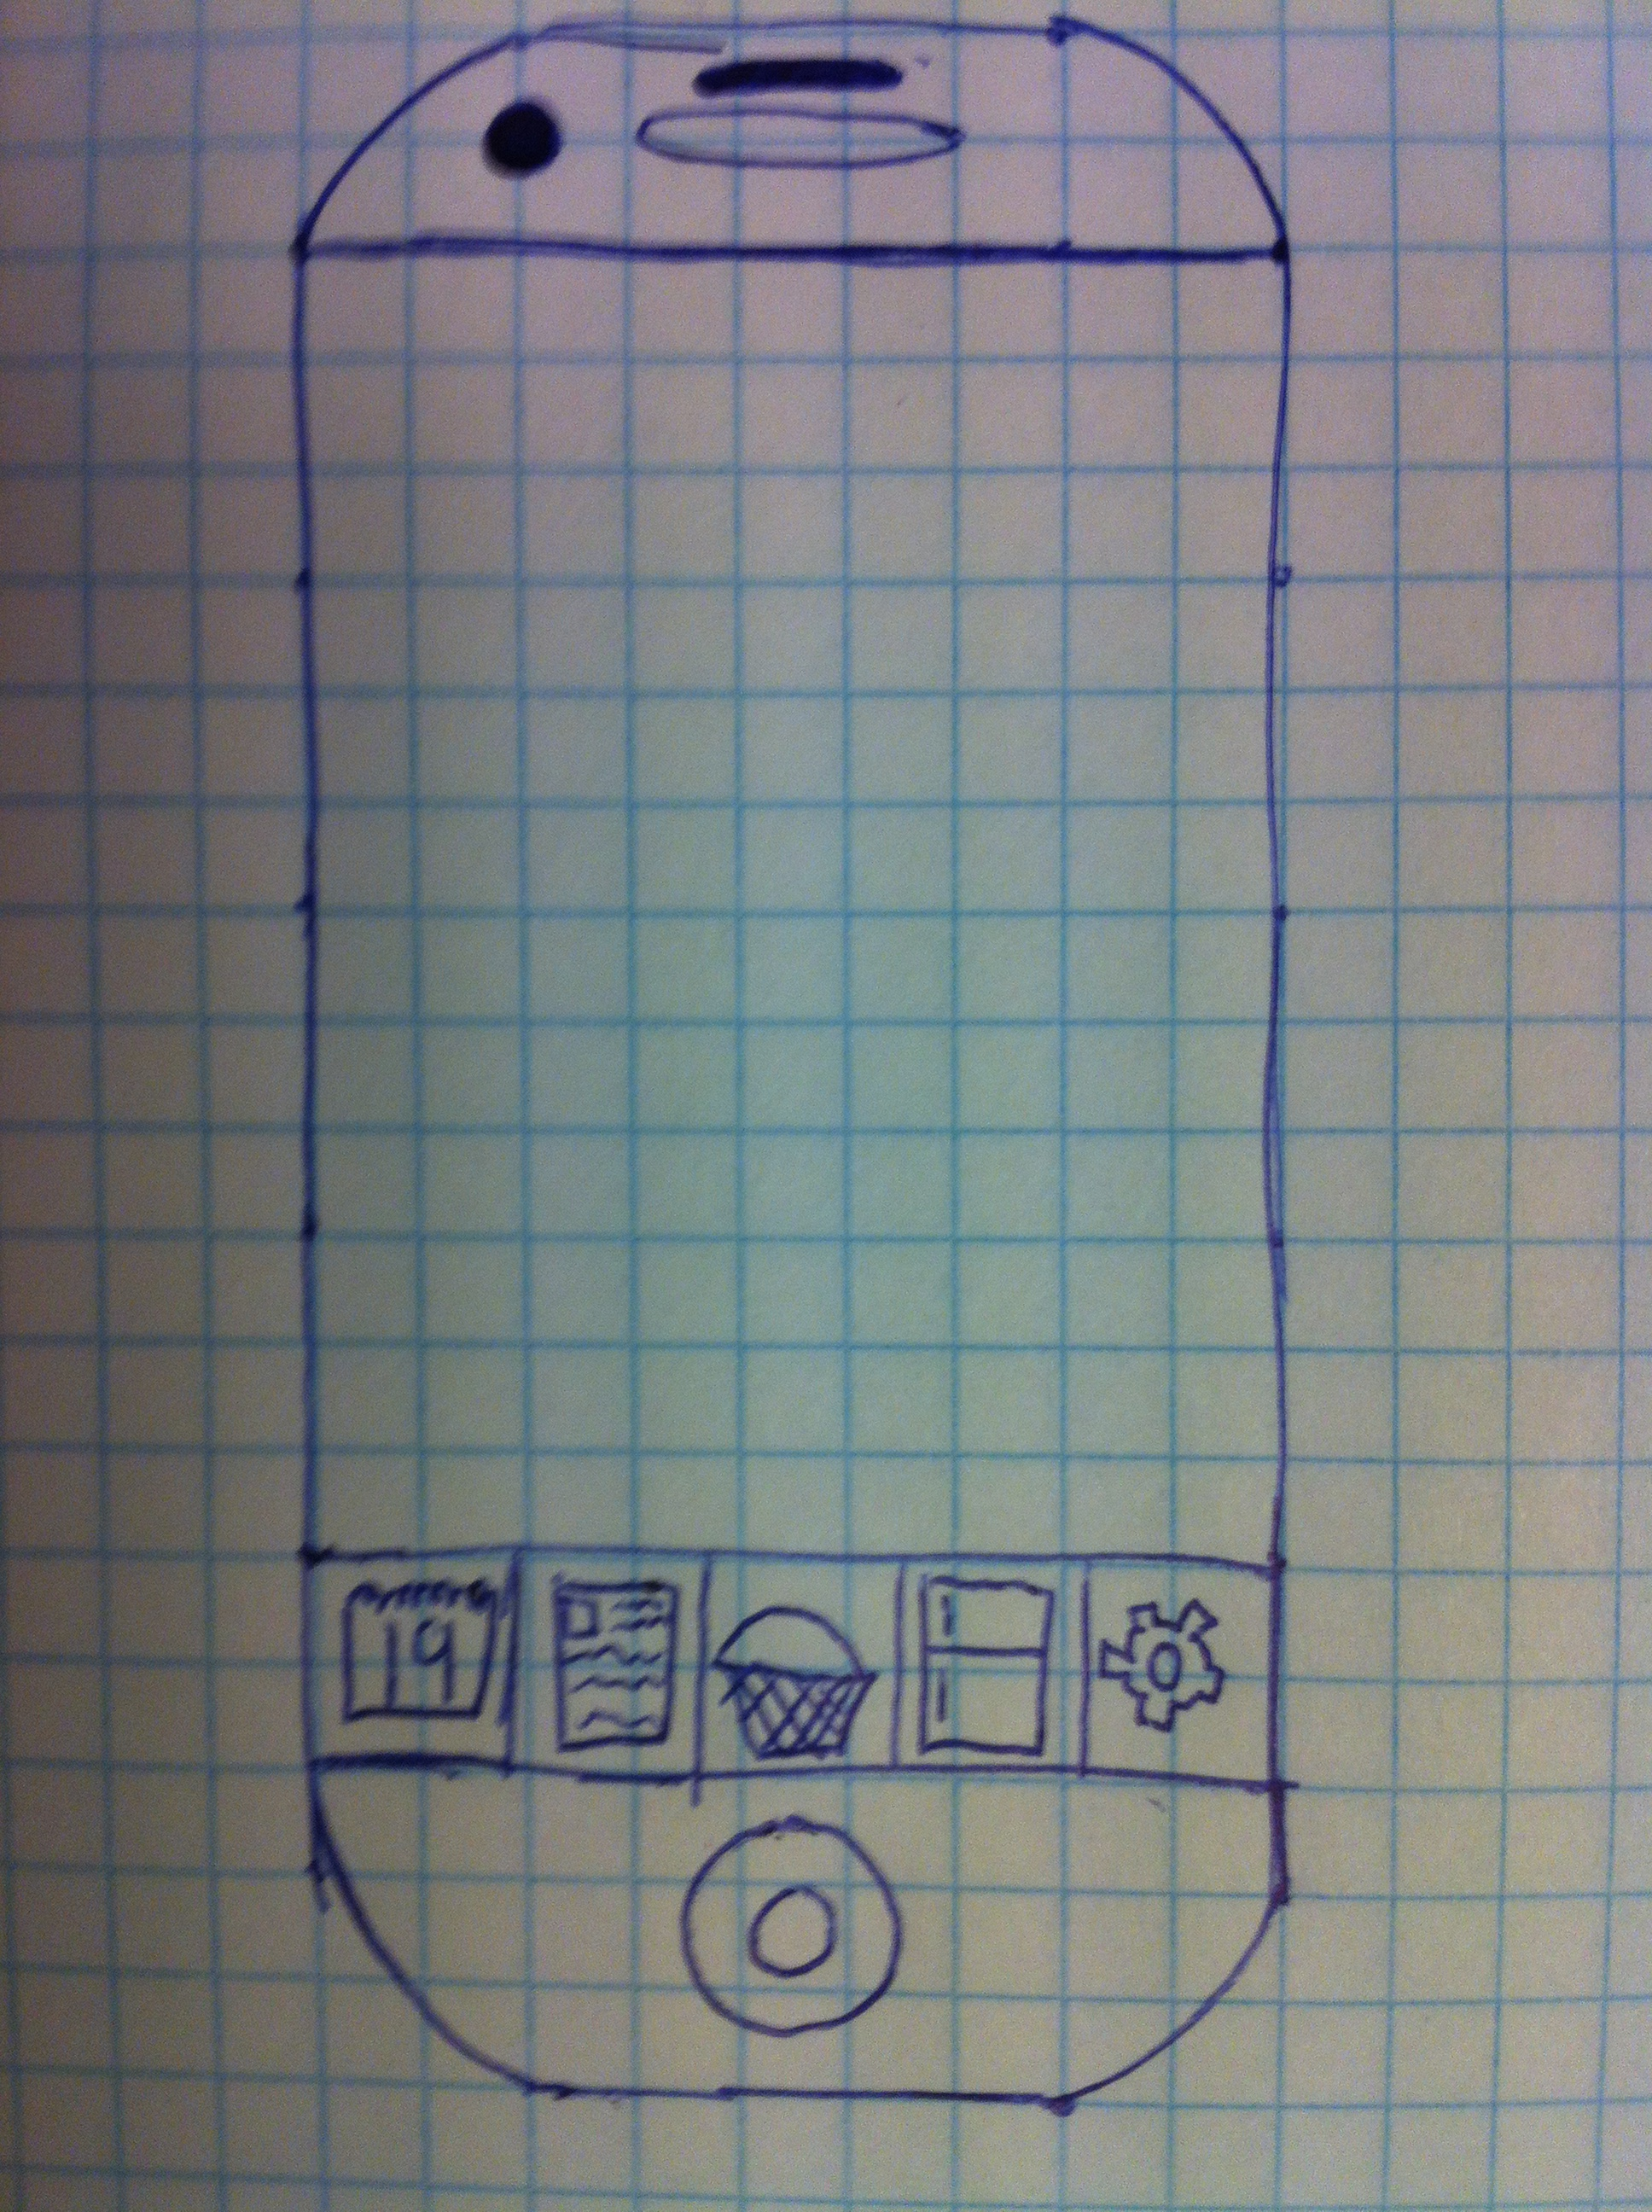
\includegraphics[width=0.5\textwidth]{Grafik/FoodPlanner/NavigationBarSketch}
	\caption{Navigation bar of the program, with the rest of the screen left blank}
	\label{NavigationBarSketch}
\end{figure}

\subsection{Navigation bar}

The navigation bar is placed in the bottom of the program, on every screen. This requires quite a large amount of space, and if the screen of the device on which the program is shown is small, the user will not have a lot of space to show the rest of the screen, therefore it has been chosen that the bar will disappear when not active.

When the user hovers over the bar, it will appear, whereas if the user does not use the navigation bar it will disappear, and only a line will be shown, so the user know that it is hidden in the bottom.

The navigation bar itself, consist of 5 element/buttons:

\begin{itemize}
    \item Meal plan
    \item Recipe
    \item Shopping list
    \item Inventory
    \item Settings
\end{itemize}

Each of the buttons take the user to the screen which it represent, and all of these screen will be described later on. The icons which are used in the representation are just for the design progress, and not necessarily the final ones.

All of the sketches, are just temporary ideas, and might be changed when they are made.